\chapter{Documenti}
\label{chap:Documenti}
Alcuni documenti.

%\newpage\mbox{}\newpage

\foreachpage{testi/lettera_fondazionale.pdf}{%
  \newpage   
  \begingroup 
    \centering
    \includegraphics[
      page=\value{imagepage},
      width=\textwidth,  
      height=\textheight,
    ]{testi/lettera_fondazionale.pdf}%
    \newpage
  \endgroup
}

%\newpage
%\begin{center}
%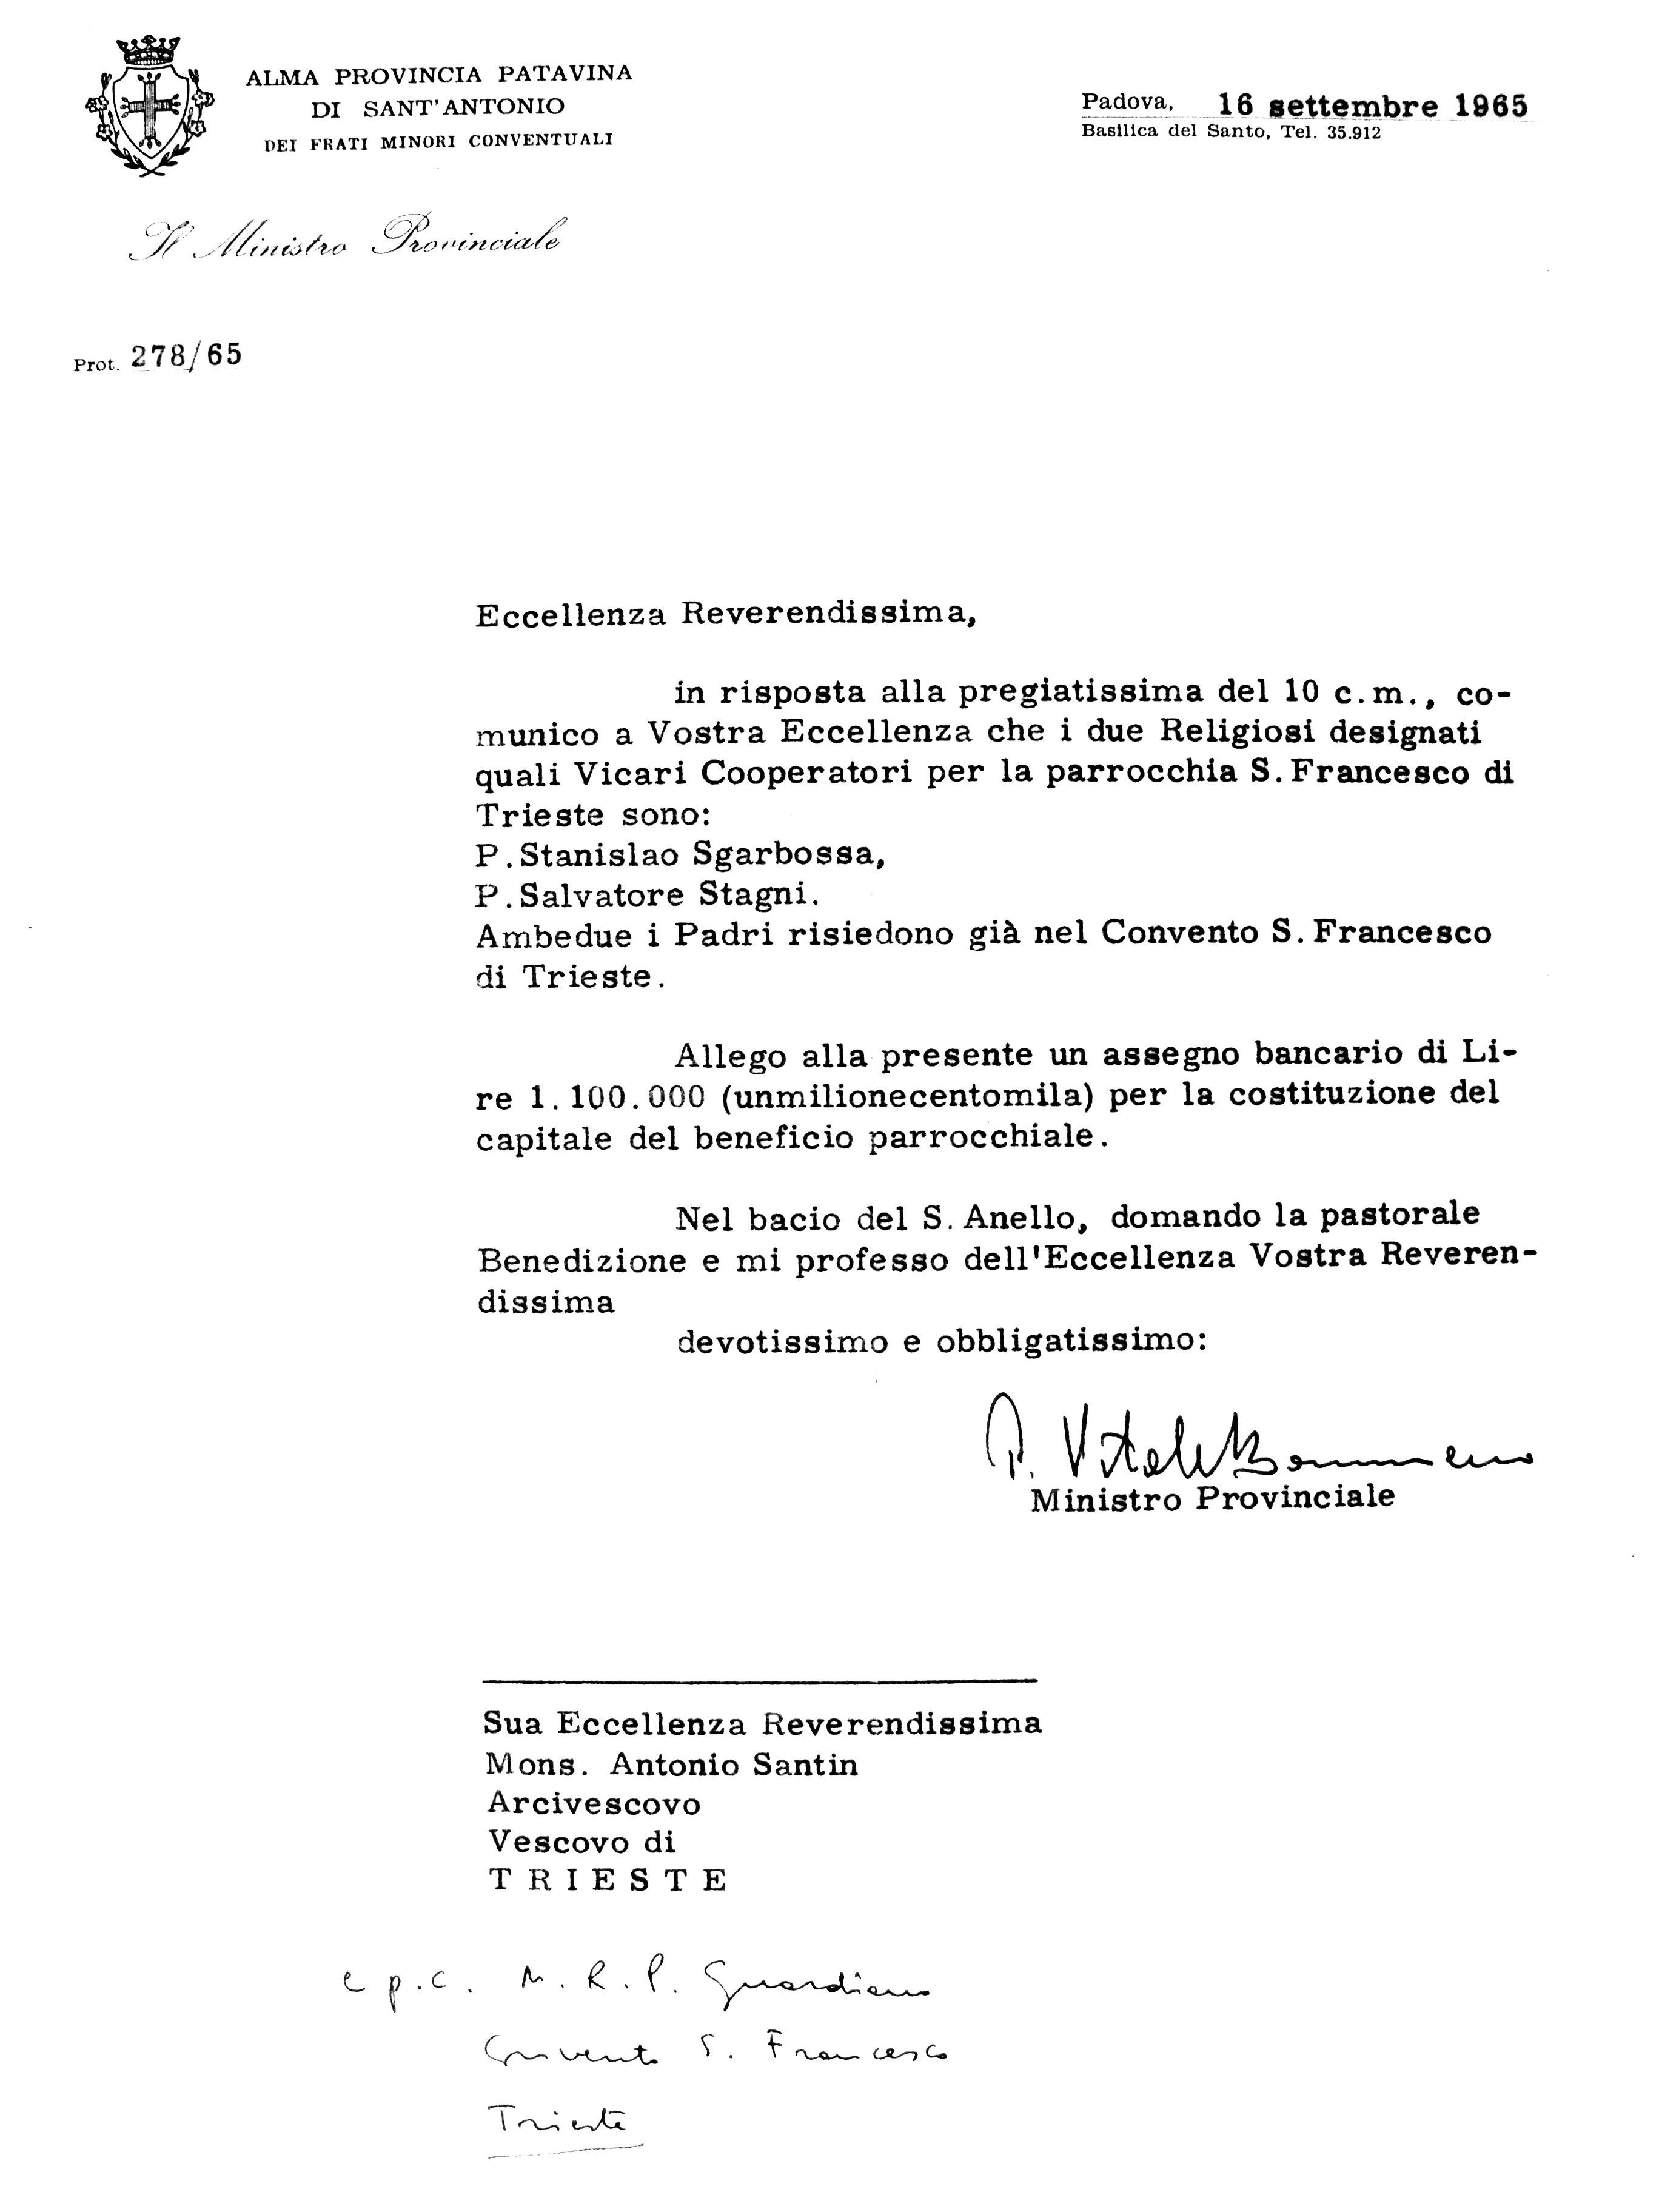
\includegraphics[
	%width=\textwidth,  
	%height=\textheight,
	%]{immagini/i_due_vicari.jpg}%
%\end{center}
%\newpage

\foreachpage{testi/riconoscimento_civile.pdf}{%
  \newpage   
  \begingroup 
    \centering
    \includegraphics[
      page=\value{imagepage},
      width=\textwidth,  
      height=\textheight,
    ]{testi/riconoscimento_civile.pdf}%
    \newpage
  \endgroup
}

\newpage
\begin{center}
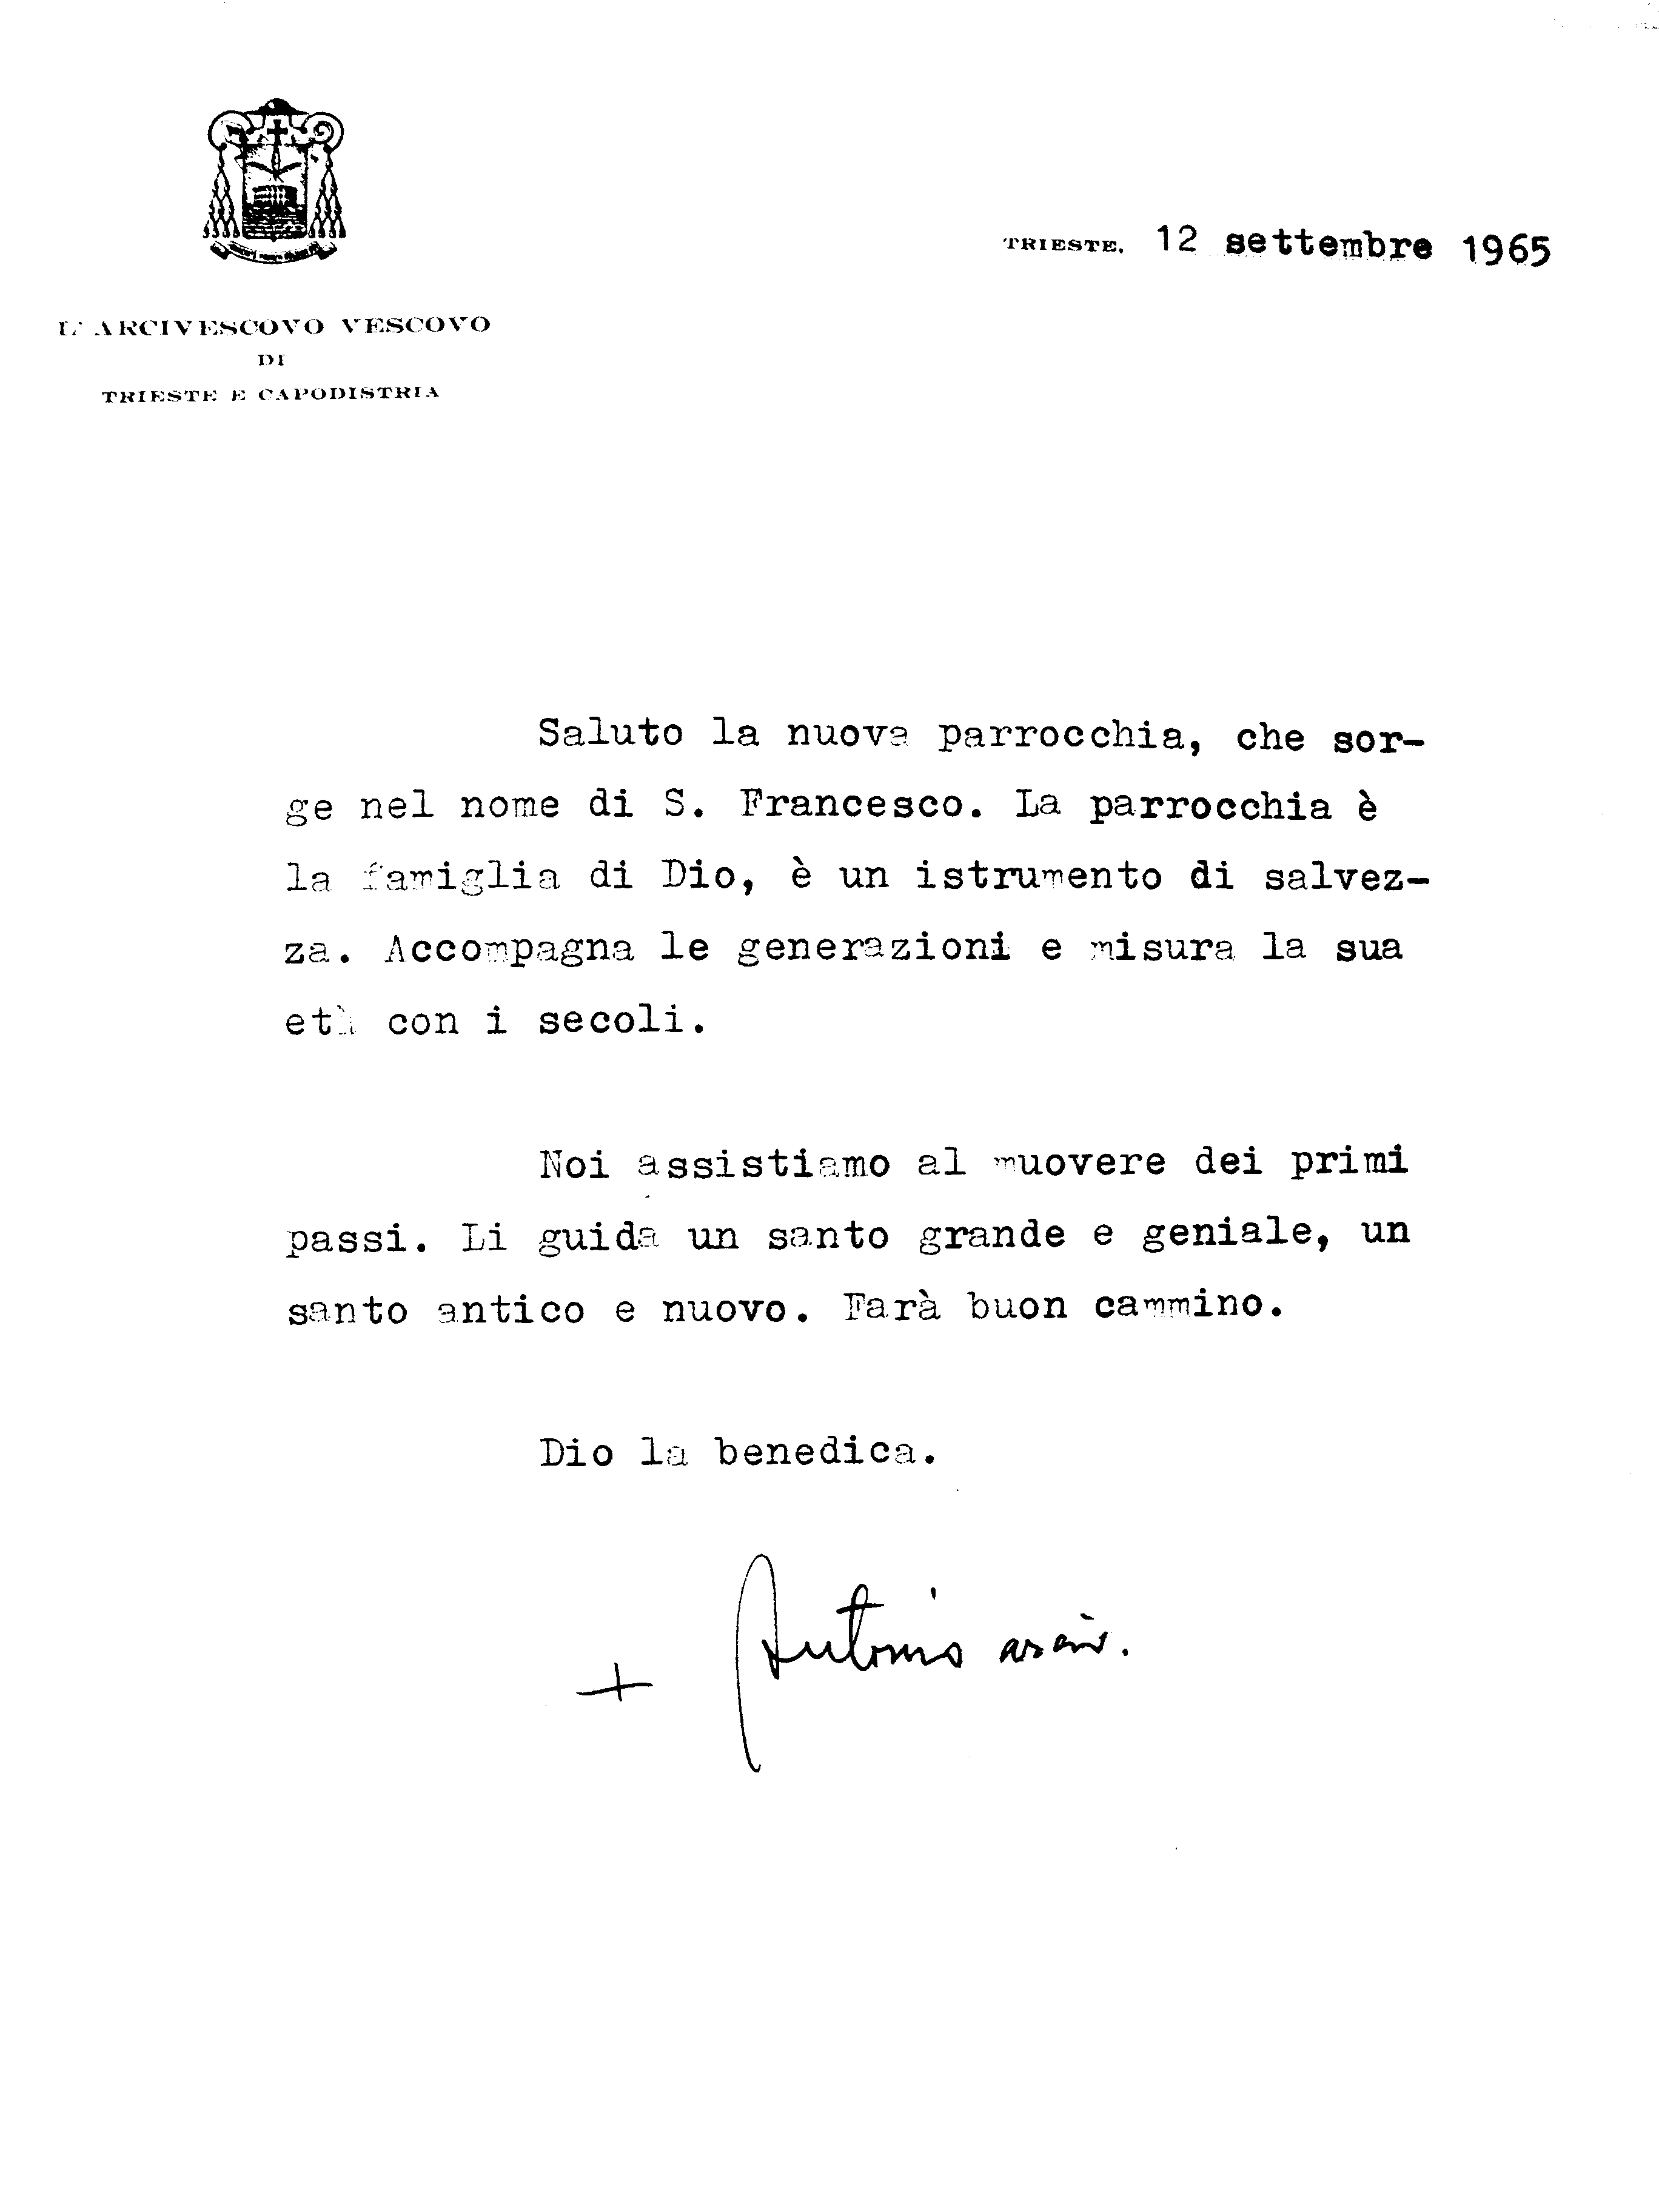
\includegraphics[
	width=\textwidth,  
	height=\textheight
	]{immagini/saluto_dal_vescovo.jpg}%
\end{center}
\newpage
\begin{center}
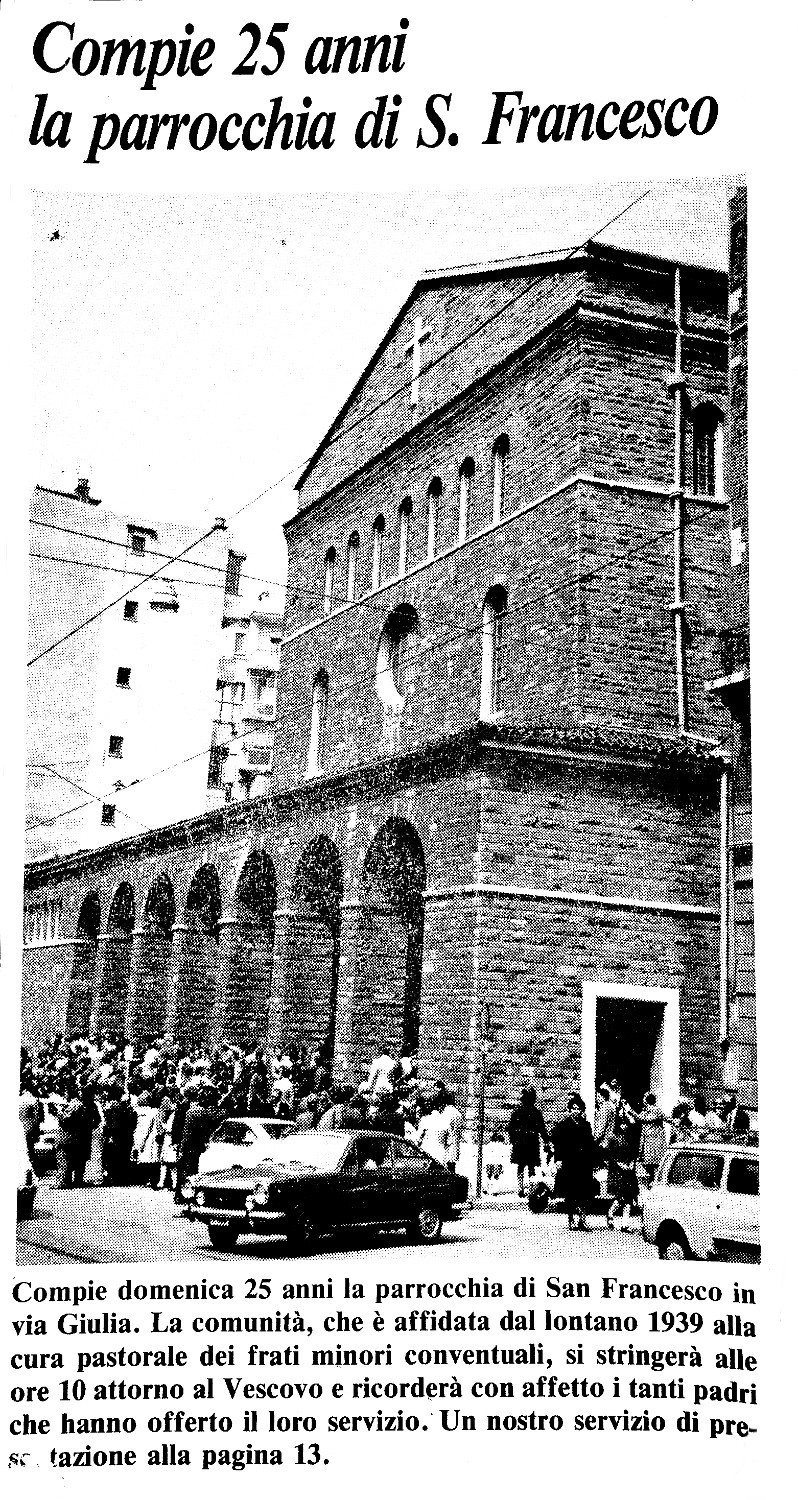
\includegraphics[
	width=\textwidth,  
	height=\textheight,
	keepaspectratio
	]{immagini/FotoParrocchia.jpg}%
\end{center}
\newpage
Il 3 maggio 1994 è stata rinnovata la Convenzione tra la Diocesi di Trieste e la Provincia Patavina OFM Conv (ora Provincia Italiana di S. Antonio di Padova) conforme le nuove indicazioni del Concilio Ecumenico Vaticano II.